
\begin{figure}[H]
    \centering
    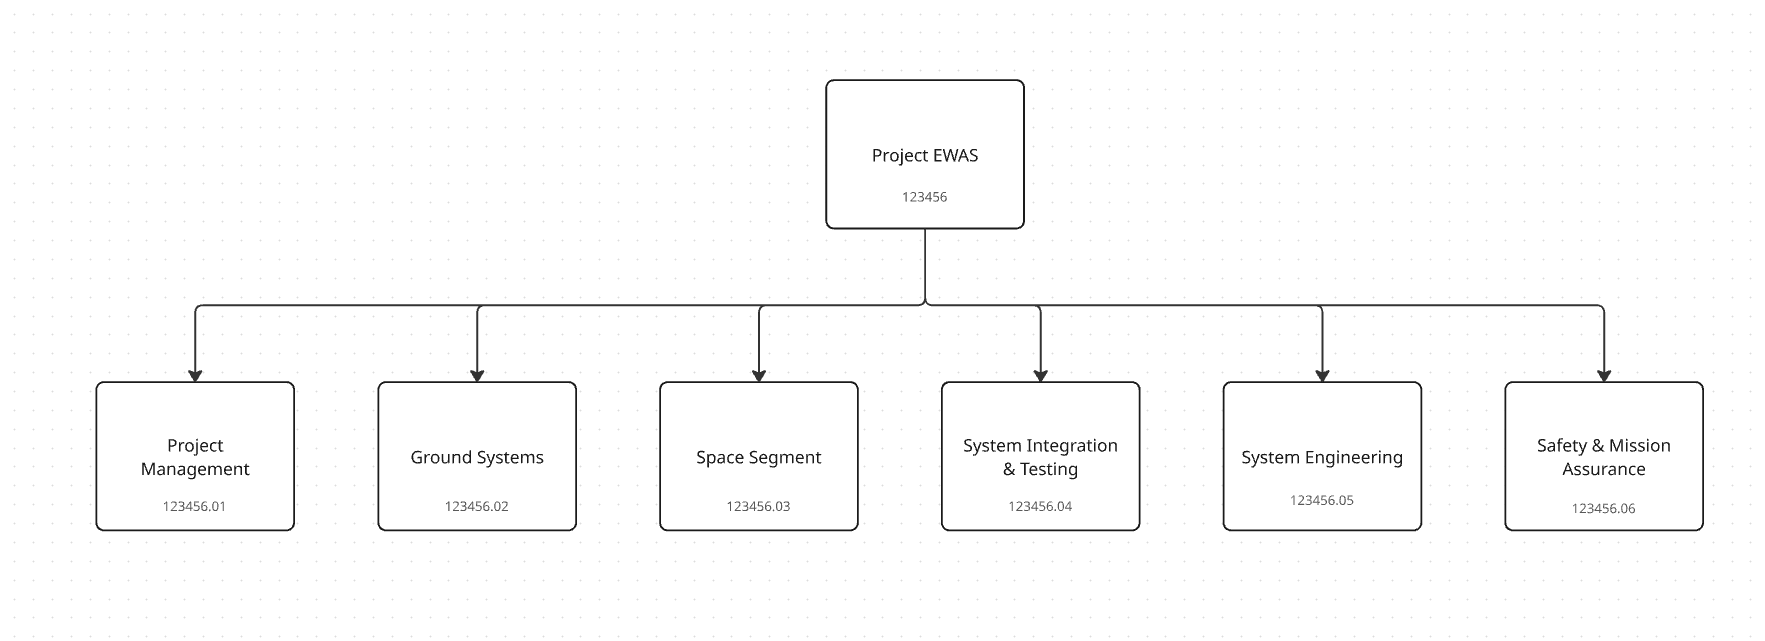
\includegraphics[width=1\textwidth]{Figures/WBS_General_LVL2.png}
    \caption{Work Breakdown Structure - Lvl 1 and Lvl 2}
    \label{fig:wbs-overview}
\end{figure}

\begin{landscape}
\begin{figure}[p]
    \centering
    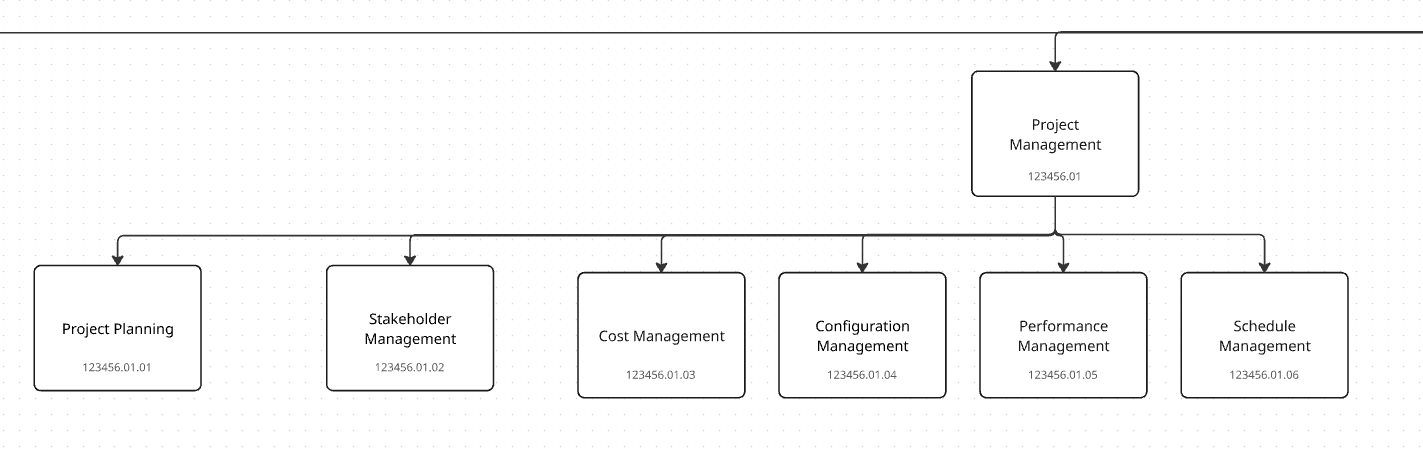
\includegraphics[width=\linewidth]{Figures/Project_Management.png}
    \caption[Project Management WBS extension]{Project Management \abbr{WBS} extension}
    \label{fig:wbs-project-management}
\end{figure}
\end{landscape}
% \textbf{Element 123456.01 - Project Management:} The management products required to
% plan, control, and monitor project execution. Includes project planning documents,
% schedules, cost baselines, performance measurement products, configuration
% management records, stakeholder management data, and project reporting
% products.\\
% \textbf{Element 123456.01.01 - Project Planning:} Products defining the overall planning
% framework for project execution. Includes project management plans and work
% breakdown structure definitions used to organize and control project scope.\\
% \textbf{Element 123456.01.01.01 - Project Management Plan:} The primary document
% describing how the project will be executed, monitored, and controlled. Includes
% scope, schedule, cost, risk, and communication planning.\\
% \textbf{Element 123456.01.01.02 - Work Breakdown Structure Definition:} The hierarchical
% decomposition of the project scope into product-oriented elements. Includes \abbr{WBS}
% structure, coding, and associated definitions.\\
% \textbf{Element 123456.01.02 - Stakeholder Management:} Products supporting
% identification, communication, and monitoring of stakeholder interactions. Includes
% stakeholder data, communication plans, and status reporting.\\
% \textbf{Element 123456.01.02.01 - Stakeholder Registry:} A documented list of identified
% stakeholders, including roles, responsibilities, and communication needs.\\
% \textbf{Element 123456.01.02.02 - Communication Plan:} Documentation defining the
% methods, frequency, and content of communication between project stakeholders.\\
% \textbf{Element 123456.01.02.03 - Status Reports:} Periodic reports summarizing project
% progress, performance, issues, and key metrics.\\
% \textbf{Element 123456.01.03 - Cost Management:} Products used to estimate, define, and
% control project costs. Includes cost baselines and cost estimation data.\\
% \textbf{Element 123456.01.03.01 - Cost Baseline:} Approved budget for the project, time-
% phased and used as a reference for cost performance measurement.\\
% \textbf{Element 123456.01.03.02 - Cost Estimates:} Quantitative assessments of the
% expected costs required to complete project work.\\
% \textbf{Element 123456.01.04 - Configuration Management:} Products used to control and
% track changes to project deliverables and documentation. Includes change records,
% configuration baselines, and control authority decisions.\\
% \textbf{Element 123456.01.04.01 - Change Request Records:} Documentation of proposed
% and approved changes to project scope, requirements, or configuration elements.\\
% \textbf{Element 123456.01.04.02 - Configuration Control Board Records:} Documentation of
% decisions and approvals made by the configuration control authority.\\
% \textbf{Element 123456.01.04.03 - Configuration Baseline:} The approved configuration of
% system elements and documentation used as a reference for change control.\\
% \textbf{Element 123456.01.05 - Performance Management:} Products used to measure and
% monitor project performance against cost, schedule, and technical baselines.
% Includes performance baselines and earned value data products.\\
% \textbf{Element 123456.01.05.01 - Performance Measurement Baseline:} The integrated
% cost and schedule baseline used for earned value analysis and performance
% tracking.\\
% \textbf{Element 123456.01.05.02 - Earned Value Reports:} Reports providing quantitative
% data on project performance, including cost and schedule variances.\\
% \textbf{Element 123456.01.06 - Schedule Management:} Products used to plan and control
% project timelines. Includes schedules and approved schedule baselines for tracking
% progress.\\
% \textbf{Element 123456.01.06.01 - Schedule Baseline:} The approved project schedule used
% as a reference for monitoring and controlling progress.\\
% \textbf{Element 123456.01.06.02 - Integrated Master Schedule:} A time-phased network of
% all project activities and milestones, used for planning, coordination, and schedule
% performance tracking.\\
\textbf{Element 123456.01 - Project Management:} The management products required to
plan, control, and monitor project execution. Includes project planning documents,
schedules, cost baselines, performance measurement products, configuration
management records, stakeholder management data, and project reporting
products.\\

\textbf{Element 123456.01.01 - Project Planning:} Products defining the overall planning
framework for project execution. Includes project management plans and work
breakdown structure definitions used to organize and control project scope.\\
\textit{Deliverables:}
\begin{itemize}
    \item Project Management Plan
    \item Project Scope and Objectives Document
    \item Project Schedule and Milestone Plan
    \item Project Risk Management Plan
    \item Work Breakdown Structure Diagram
    \item WBS Dictionary
    \item WBS Coding Structure
\end{itemize}

\textbf{Element 123456.01.02 - Stakeholder Management:} Products supporting
identification, communication, and monitoring of stakeholder interactions. Includes
stakeholder data, communication plans, and status reporting.\\
\textit{Deliverables:}
\begin{itemize}
    \item Stakeholder Register
    \item Stakeholder Roles and Responsibilities Matrix
    \item Project Communication Plan
    \item Project Communication Matrix
    \item Stakeholder Communication Schedule
    \item Periodic Project Progress Reports
    \item Project Issues and Actions Log
    \item Milestone Review Reports
\end{itemize}

\textbf{Element 123456.01.03 - Cost Management:} Products used to estimate, define, and
control project costs. Includes cost baselines and cost estimation data.\\
\textit{Deliverables:}
\begin{itemize}
    \item Project Cost Baseline
    \item Time-Phased Budget Allocation
    \item Preliminary Project Cost Estimate
    \item Cost Estimation Assumptions and Basis
    \item Cost Breakdown by Major Project Elements
\end{itemize}

\textbf{Element 123456.01.04 - Configuration Management:} Products used to control and
track changes to project deliverables and documentation. Includes change records,
configuration baselines, and control authority decisions.\\
\textit{Deliverables:}
\begin{itemize}
    \item Change Request Log
    \item Change Impact Assessment Records
    \item Change Approval and Rejection Records
    \item Configuration Control Board Meeting Minutes
    \item Configuration Change Decision Log
    \item Approved Document Baseline
    \item System Configuration Baseline
    \item Configuration Item Register
\end{itemize}

\textbf{Element 123456.01.05 - Performance Management:} Products used to measure and
monitor project performance against cost, schedule, and technical baselines.
Includes performance baselines and earned value data products.\\
\textit{Deliverables:}
\begin{itemize}
    \item Performance Measurement Baseline
    \item Project Performance Indicators and Metrics
    \item Earned Value Management Reports
    \item Cost and Schedule Variance Reports
    \item Project Performance Trend Analysis
\end{itemize}

\textbf{Element 123456.01.06 - Schedule Management:} Products used to plan and control
project timelines. Includes schedules and approved schedule baselines for tracking
progress.\\
\textit{Deliverables:}
\begin{itemize}
    \item Approved Project Schedule Baseline
    \item Project Milestone Schedule
    \item Integrated Master Schedule (IMS)
    \item Project Activity Dependency Network
    \item Critical Path Analysis Report
\end{itemize}

\begin{landscape}
\begin{figure}[p]
    \centering
    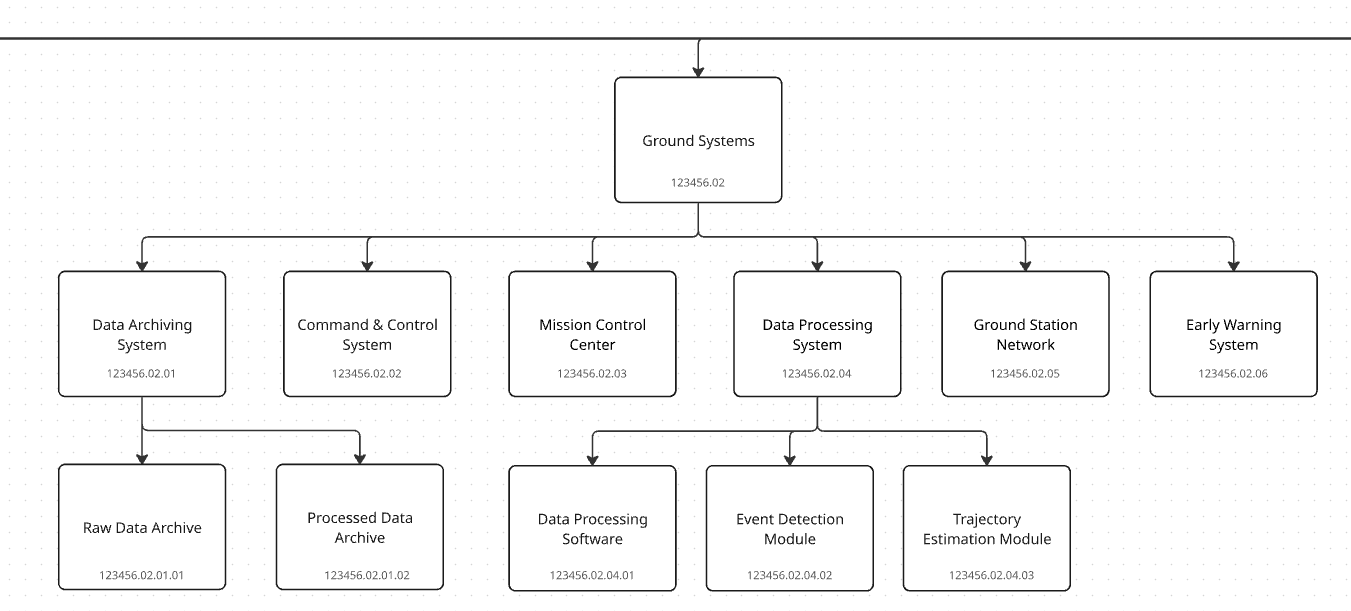
\includegraphics[width=\linewidth]{Figures/Ground_Systems.png}
    \caption{Ground Systems extension}
    \label{fig:wbs-ground-systems}
\end{figure}
\end{landscape}
\textbf{Element 123456.02 - Ground Systems:} The systems, facilities, software, and
networks required to operate the space segment and support mission execution.
Includes command and control, data processing, data archiving, ground station
infrastructure, and mission-specific operational systems such as early warning
capabilities.\\
\textbf{Element 123456.02.01 - Data Archiving System:} System responsible for storage,
management, and retrieval of mission data. Includes infrastructure for handling raw
and processed data products generated during mission operations.\\
\textbf{Element 123456.02.01.01 - Raw Data Archive:} Repository for unprocessed mission
data received from spacecraft systems and ground stations. Includes storage of
telemetry, sensor outputs, and initial acquisition data.\\
\textbf{Element 123456.02.01.02 - Processed Data Archive:} Repository for processed and
analyzed data products derived from raw mission data. Includes refined datasets
used for mission analysis and operational decision-making.\\
\textbf{Element 123456.02.02 - Command \& Control System:} System responsible for
generation, transmission, and management of commands sent to the spacecraft, as
well as monitoring and control of spacecraft operations. Includes command
interfaces and control software.\\
\textbf{Element 123456.02.03 - Mission Control Center:} Facility and associated systems
used for monitoring spacecraft status, executing mission operations, and
coordinating ground system activities. Includes operator interfaces, monitoring
systems, and operational control tools.\\
\textbf{Element 123456.02.04 - Data Processing System:} System responsible for
processing, transforming, and analyzing mission data received from the spacecraft.
Includes software and algorithms required to extract meaningful information for
mission operations.\\
\textbf{Element 123456.02.04.01 - Data Processing Software:} Software responsible for
ingestion, conditioning, and transformation of raw data into formats suitable for
analysis. Includes preprocessing, filtering, and data preparation functions.\\
\textbf{Element 123456.02.04.02 - Event Detection Module:} Software module responsible
for identifying significant events within processed data, such as launch detection or
anomaly identification.\\
\textbf{Element 123456.02.04.03 - Trajectory Estimation Module:} Software module
responsible for estimating object trajectories based on processed data inputs.
Includes algorithms for calculating position, velocity, and predicted paths.\\
\textbf{Element 123456.02.05 - Ground Station Network:} Network of ground-based stations
used to communicate with the spacecraft. Includes antennas, communication links,
and supporting infrastructure for telemetry reception and command transmission.\\
\textbf{Element 123456.02.06 - Early Warning System:} System responsible for generating
and disseminating alerts based on analyzed mission data. Includes components for
event classification, alert generation, and communication of warning information to
external users or systems.\\
\begin{landscape}
\begin{figure}[p]
    \centering
    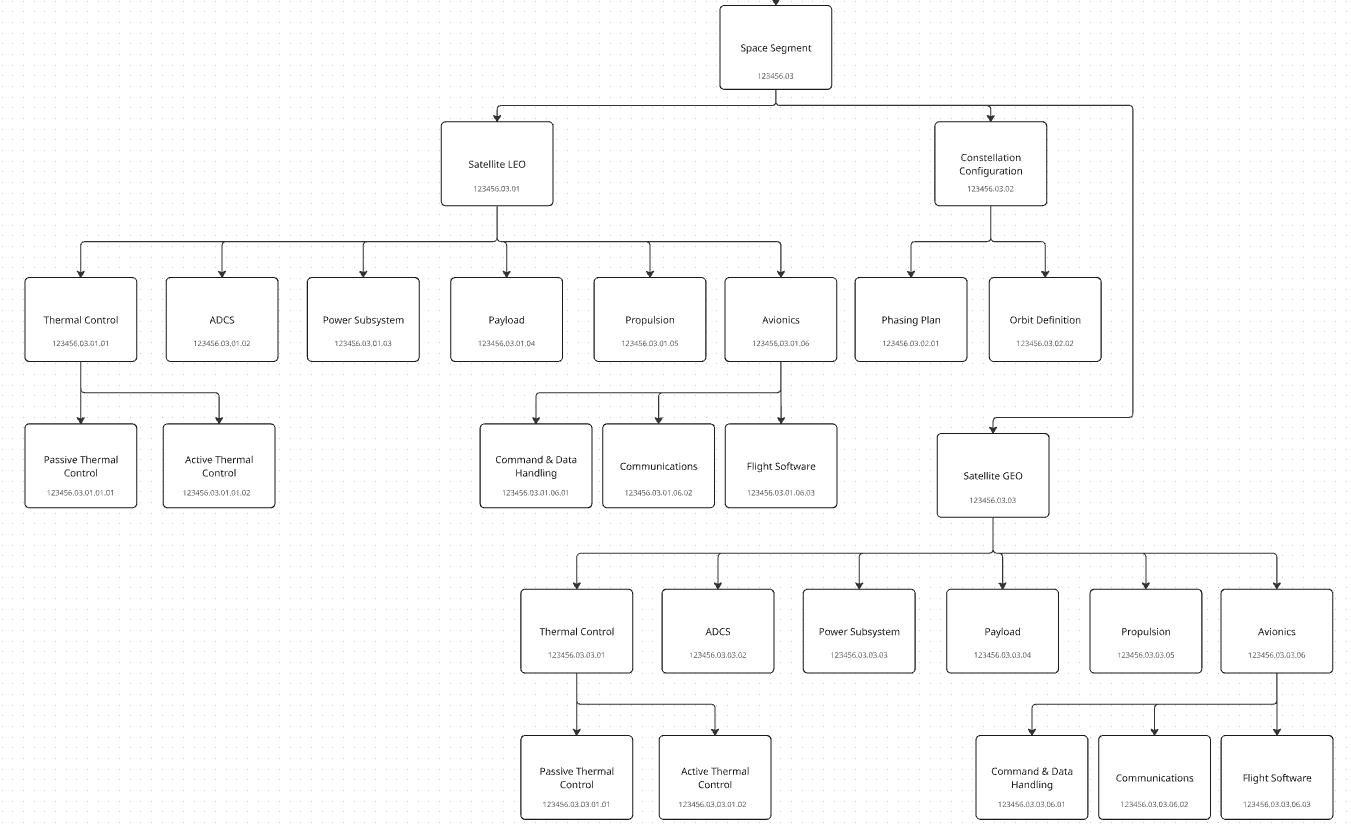
\includegraphics[width=\linewidth]{Figures/Space_Segment.png}
    \caption{Space Segment extension}
    \label{fig:wbs-space-segment}
\end{figure}
\end{landscape}
\textbf{Element 123456.03 - Space Segment:} The hardware and software elements
required to perform the space-based mission functions. This includes the satellite
system and constellation configuration defining orbital parameters and satellite
distribution.\\
\textbf{Element 123456.03.01 - Satellite:} The flight system consisting of all onboard
subsystems required to support mission operations in orbit. Includes payload,
spacecraft bus subsystems, avionics, propulsion, and flight software.\\
\textbf{Element 123456.03.01.01 - Thermal Control:} Subsystem responsible for maintaining
spacecraft temperature within operational limits. Includes passive and active thermal
control components and associated hardware.\\
\textbf{Element 123456.03.01.01.01 - Passive Thermal Control:} Subsystem components
that maintain spacecraft temperature within acceptable limits without active power
consumption. Includes thermal coatings, insulation (\abbr{MLI}), radiators, and structural
thermal design features.\\
\textbf{Element 123456.03.01.01.02 - Active Thermal Control:} Subsystem components that
regulate spacecraft temperature using powered devices. Includes heaters,
thermostats, fluid loops, heat pipes, and associated control electronics.\\
\textbf{Element 123456.03.01.02 - Attitude Determination and Control System (\abbr{ADCS}):}
Subsystem providing spacecraft orientation determination and control. Includes
sensors, actuators, and control algorithms required for pointing and stabilization.\\
\textbf{Element 123456.03.01.03 - Power Subsystem:} Subsystem responsible for
generation, storage, conditioning, and distribution of electrical power, including solar
arrays, batteries, and power management electronics.\\
\textbf{Element 123456.03.01.04 - Payload:} Mission-specific instruments and sensors
responsible for detection and data acquisition required to fulfill mission objectives.\\
\textbf{Element 123456.03.01.05 - Propulsion Subsystem:} Subsystem providing thrust for
orbit insertion, maintenance, and maneuvering, including thrusters, propellant
storage, and associated control components.\\
\textbf{Element 123456.03.01.06 - Avionics:} Onboard electronic systems responsible for
command, data processing, communication, and software execution.\\
\textbf{Element 123456.03.01.06.01 - Command \& Data Handling (\abbrtext{CDH}{C\&DH}):} Subsystem
responsible for onboard data processing, command execution, and data
management. Includes onboard computers, data buses, memory units, and
associated control software required for spacecraft operations.\\
\textbf{Element 123456.03.01.06.02 - Communications:} Subsystem responsible for
transmission and reception of telemetry, tracking, and command (\abbrtext{TTC}{TT\&C}) data
between the spacecraft and ground systems. Includes antennas, transceivers, \abbr{RF}
components, and communication protocols.\\
\textbf{Element 123456.03.01.06.03 - Flight Software:} Software executed onboard the
spacecraft to control system functions, manage subsystem operations, process data,
and execute mission tasks. Includes control algorithms, fault management, and
operational logic.\\
\textbf{Element 123456.03.02 - Constellation Configuration:} Definition of the orbital
architecture and spatial distribution of satellites within the constellation, including
orbital parameters and phasing.\\
\textbf{Element 123456.03.02.01 - Constellation Phasing Plan:} The definition of satellite
distribution and relative positioning within orbital planes to ensure required coverage
and mission performance.\\
\textbf{Element 123456.03.02.02 - Orbit Definition:} The specification of orbital parameters
including altitude, inclination, eccentricity, and orbital plane configuration.

\begin{landscape}
\begin{figure}[p]
    \centering
    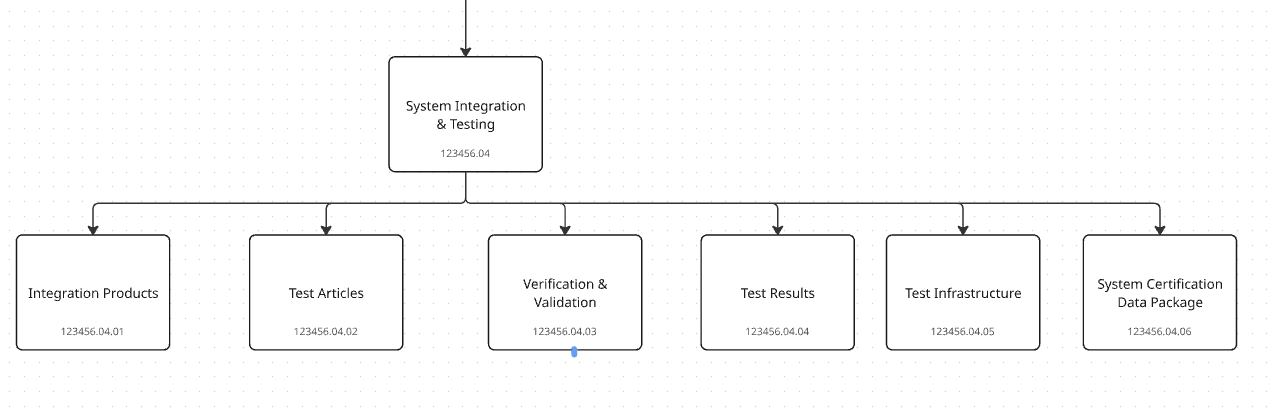
\includegraphics[width=\linewidth]{Figures/System_Integration_and_Testing.png}
    \caption{System Integration \& Testing extension}
    \label{fig:wbs-integration-testing}
\end{figure}
\end{landscape}
\textbf{Element 123456.04 - Systems Integration and Testing:} This element includes the
products, data, and supporting infrastructure required to integrate system
components and verify system performance against requirements.\\
\textbf{Element 123456.04.01 - Integration Products:} Integrated hardware and software
system configurations resulting from assembly and integration activities. Includes
system-level configurations combining space, ground, and interface elements
required for testing and verification.\\
\textbf{Element 123456.04.02 - Test Articles:} Physical system models and configurations
used for verification and testing. Includes engineering, qualification, and flight models
representing different stages of system maturity.\\
\textbf{Element 123456.04.02.01 - Qualification Model:} A representative model used to
demonstrate compliance with environmental and performance requirements under
qualification test conditions.\\
\textbf{Element 123456.04.02.02 - Engineering Model:} A non-flight configuration used for
design verification, integration testing, and functional validation during development.\\
\textbf{Element 123456.04.02.03 - Flight Model:} The flight-ready system configuration
intended for operational deployment and mission execution.\\
\textbf{Element 123456.04.03 - Verification \& Validation Products:} Documentation and data
products demonstrating compliance with system requirements and validation of
mission objectives. Includes traceability matrices and validation reports.\\
\textbf{Element 123456.04.03.01 - Verification Matrix:} A structured data product mapping
system requirements to verification methods and test results, providing evidence of
requirement compliance.\\
\textbf{Element 123456.04.03.02 - Validation Reports:} Documentation confirming that the
system meets intended operational goals and mission objectives under realistic
conditions.\\
\textbf{Element 123456.04.04 - Test Results:} Documented outcomes of system-level and
subsystem-level testing activities. Includes environmental, functional, and
performance test results demonstrating system behavior.\\
\textbf{Element 123456.04.05 - Test Infrastructure:} Facilities, equipment, and tools required
to support system integration and testing. Includes ground support equipment, test
benches, and simulation environments.\\
\textbf{Element 123456.04.05.01 - Test Benches:} Dedicated test setups configured to
evaluate specific subsystems or functions. Includes hardware and software
environments supporting functional and integration testing.\\
\textbf{Element 123456.04.05.02 - Ground Support Equipment:} Equipment used to support
testing, integration, and operation of the system from the ground. Includes electrical
and mechanical interfaces, control systems, and support hardware.\\
\textbf{Element 123456.04.05.03 - Simulators:} Software or hardware systems used to
emulate spacecraft, environment, or mission conditions for testing and validation
purposes.\\
\textbf{Element 123456.04.06 - System Certification Data Package:} A compiled set of
verification, validation, and test data used to demonstrate system compliance with
requirements and readiness for operational use. Includes supporting evidence from
test results, analysis, and verification activities.
\begin{landscape}
\begin{figure}[p]
    \centering
    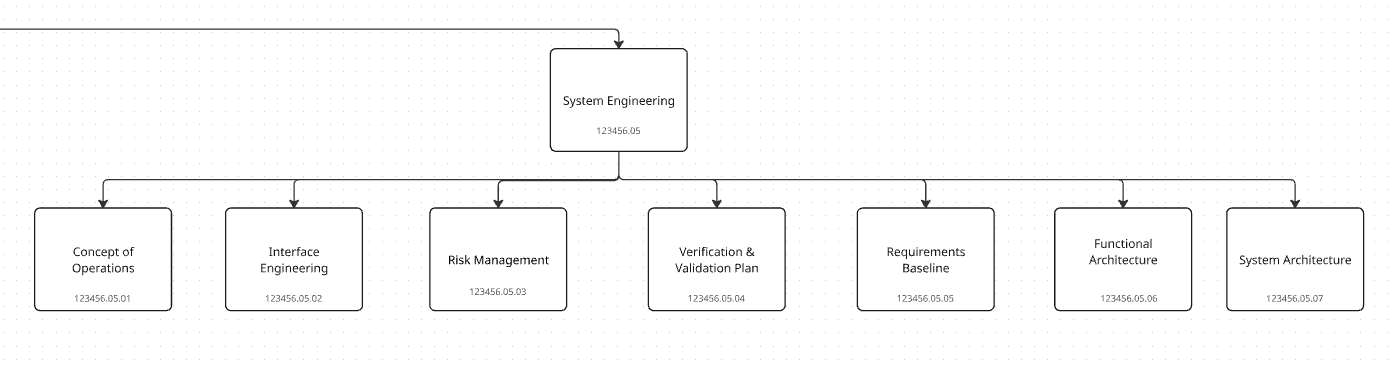
\includegraphics[width=\linewidth]{Figures/System_Engineering.png}
    \caption{System Engineering extension}
    \label{fig:wbs-system-engineering}
\end{figure}
\end{landscape}
\textbf{Element 123456.05 - Systems Engineering:} The products required to define,
integrate, and verify the technical baseline of the system. Includes requirements
documentation, system architecture descriptions, interface control documents,
verification and validation plans, risk management products, and concept of
operations documentation.\\
\textbf{Element 123456.05.01 - Concept of Operations Document:} A document describing
how the system is intended to operate in its mission environment. Includes
operational scenarios, system interactions, and end-to-end mission workflows.\\
\textbf{Element 123456.05.02 - Interface Control Documents:} Documentation defining
interfaces between system elements. Includes interface specifications for data
exchange, external systems, and segment-level interactions.\\
\textbf{Element 123456.05.02.01 - Data Exchange Interface Control Document:}
Documentation defining data formats, protocols, and interfaces for information
exchange between system components.\\
\textbf{Element 123456.05.02.02 - External Systems Interface Control Document:}
Documentation defining interfaces between the system and external entities or
partner systems.\\
\textbf{Element 123456.05.02.03 - Ground Segment Interface Control Document:}
Documentation defining interfaces within the ground system and between ground
and other system elements.\\
\textbf{Element 123456.05.02.04 - Space Segment Interface Control Document:}
Documentation defining interfaces within the space segment and between spacecraft
subsystems.\\
\textbf{Element 123456.05.03 - Risk Management:} Products used to identify, analyze,
track, and mitigate project risks. Includes risk register, risk assessment results,
mitigation plans, and risk reporting products.\\
\textbf{Element 123456.05.03.03 - Risk Register:} A structured repository of identified risks,
including descriptions, probabilities, impacts, and status.\\
\textbf{Element 123456.05.03.04 - Risk Assessment Results:} Documented evaluation of
risks, including probability and impact analysis results.\\
\textbf{Element 123456.05.03.04.01 - Probability Scale Definition:} Definition of probability
levels used to assess risks consistently across the project.\\
\textbf{Element 123456.05.03.04.02 - Impact Assessment Results:} Evaluation of potential
consequences associated with identified risks.\\
\textbf{Element 123456.05.03.02 - Risk Mitigation Plans:} Documentation defining strategies
and actions to reduce risk probability and impact, including contingency approaches.\\
\textbf{Element 123456.05.03.01 - Risk Status Reports:} Reports providing updates on risk
status, mitigation progress, and risk trends.\\
\textbf{Element 123456.05.03.01.01 - Risk Tracking Reports:} Data products monitoring
changes in risk status over time.\\
\textbf{Element 123456.05.03.01.02 - Risk Review Reports:} Documentation of periodic risk
reviews and associated decisions.\\
\textbf{Element 123456.05.04 - Verification \& Validation Plan:} Documentation defining the
methods, processes, and criteria used to verify and validate system performance
against requirements.\\
\textbf{Element 123456.05.05 - Requirements Baseline:} The complete set of approved
system and mission requirements, including traceability and supporting
documentation.\\
\textbf{Element 123456.05.05.01 - Requirements Traceability Matrix:} A structured mapping
between requirements and their verification methods and implementation elements.\\
\textbf{Element 123456.05.05.02 - System Requirements Document:} Documentation
defining technical requirements for system design and implementation.\\
\textbf{Element 123456.05.05.03 - Mission Requirements Document:} Documentation
defining high-level mission objectives and constraints.\\
\textbf{Element 123456.05.06 - Functional Architecture Model:} Representation of system
functions and their relationships, describing how system processes are organized
and interact.\\
\textbf{Element 123456.05.07 - System Architecture Description:} Documentation describing
the physical and logical structure of the system, including components, interfaces,
and interactions.
\begin{landscape}
\begin{figure}[p]
    \centering
    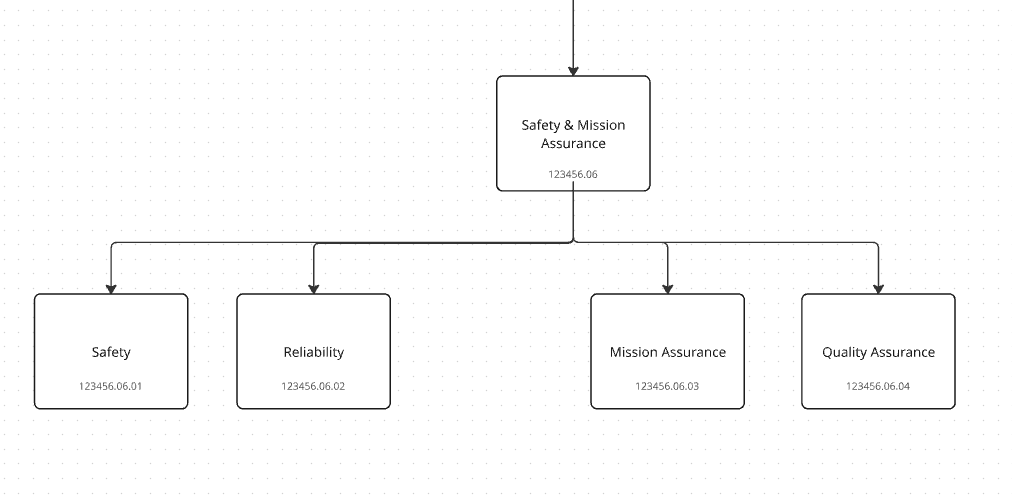
\includegraphics[width=\linewidth]{Figures/Safety_and_Mission_Assurance.png}
    \caption{Safety \& Mission Assurance extension}
    \label{fig:wbs-safety-assurance}
\end{figure}
\end{landscape}
\textbf{Element 123456.06 - Safety \& Mission Assurance:} The products required to ensure
system safety, reliability, quality, and mission success. Includes safety data products,
reliability analysis results, quality assurance records, and certification documentation
required to demonstrate system compliance and readiness.\\
\textbf{Element 123456.06.01 - Safety:} Products related to identification, evaluation, and
control of hazards to ensure system safety. Includes hazard analysis data, safety
tracking systems, and safety review documentation.\\
\textbf{Element 123456.06.01.01 - Hazard Analysis Report:} Documentation identifying
potential hazards, their causes, and associated mitigation measures to ensure safe
system operation.\\
\textbf{Element 123456.06.01.02 - Safety Review Data Package:} A collection of safety-
related documentation supporting safety reviews, including hazard analysis and
compliance evidence.\\
\textbf{Element 123456.06.01.03 - Hazard Tracking System:} A system used to monitor and
manage identified hazards, including status, mitigation actions, and closure records.\\
\textbf{Element 123456.06.02 - Reliability:} Products related to assessment and prediction
of system reliability. Includes reliability analysis results, failure data, and modeling
outputs.\\
\textbf{Element 123456.06.02.01 - Reliability Prediction:} Analytical results estimating
system reliability metrics such as failure rates and mean time between failures.\\
\textbf{Element 123456.06.02.02 - \abbr{FMEA} and Fault Tree Analysis Results:} Analysis results
identifying failure modes, their effects, and system-level fault propagation.\\
\textbf{Element 123456.06.02.03 - Failure Reports:} Documentation describing system
failures, anomalies, and associated root cause analysis.\\
\textbf{Element 123456.06.03 - Mission Assurance:} Products ensuring that the system
meets mission success criteria and operational requirements. Includes certification
documentation, compliance evidence, and readiness support materials.\\
\textbf{Element 123456.06.03.01 - Flight Readiness Review Data Package:} Documentation
supporting the evaluation of system readiness for operational deployment.\\
\textbf{Element 123456.06.03.02 - Compliance Verification Evidence:} Documented
evidence demonstrating that system requirements and standards have been met.\\
\textbf{Element 123456.06.03.03 - Final Certification Package:} The approved
documentation set confirming system compliance and readiness for operational use.\\
\textbf{Element 123456.06.04 - Quality Assurance:} Products used to ensure that system
development and manufacturing comply with defined standards. Includes inspection
records, audit reports, and nonconformance documentation.\\
\textbf{Element 123456.06.04.01 - Inspection Record:} Documentation of inspections
performed on hardware, software, or processes to verify compliance with
requirements.\\
\textbf{Element 123456.06.04.02 - Quality Assurance Audit Reports:} Reports documenting
results of audits conducted to verify compliance with quality standards and
procedures.\\
\textbf{Element 123456.06.04.03 - Nonconformance Reports:} Documentation of deviations
from requirements, including descriptions, impacts, and corrective actions.